\subsection{Previous courses page (Vlad)}

This page offers an overview for the courses the student took previously, grouped by semester. The previous courses page is very similar in design to the current courses page, with addition of simple marks to indicate whether the student passed or failed the completed course, and a tab bar to navigate through previous semesters.\\
All the courses are presented in a table each row being separated by a new line for better understanding of the page. Each course has a default picture so the user can easily find the desired course in the list. \\
The semester list grows horizontally because it can be compacted better than the list of courses, is less likely to be used, and because it is more difficult to scroll horizontally than vertically on most computers. A less-used feature should use the more difficult action, leaving more natural actions for commonly used features.\\
Orienting the list of semesters horizontally versus the vertical orientation of the courses helps reinforce that the user is navigating through a different set of information than when they simply scroll through courses.\\
Each course has as information the final grade which was obtained by the student and a check mark if it was a passing grade. If the grade is below 45\% the sign changes to a red cross. This can be seen for GenCS where the grade is 35\%.\\
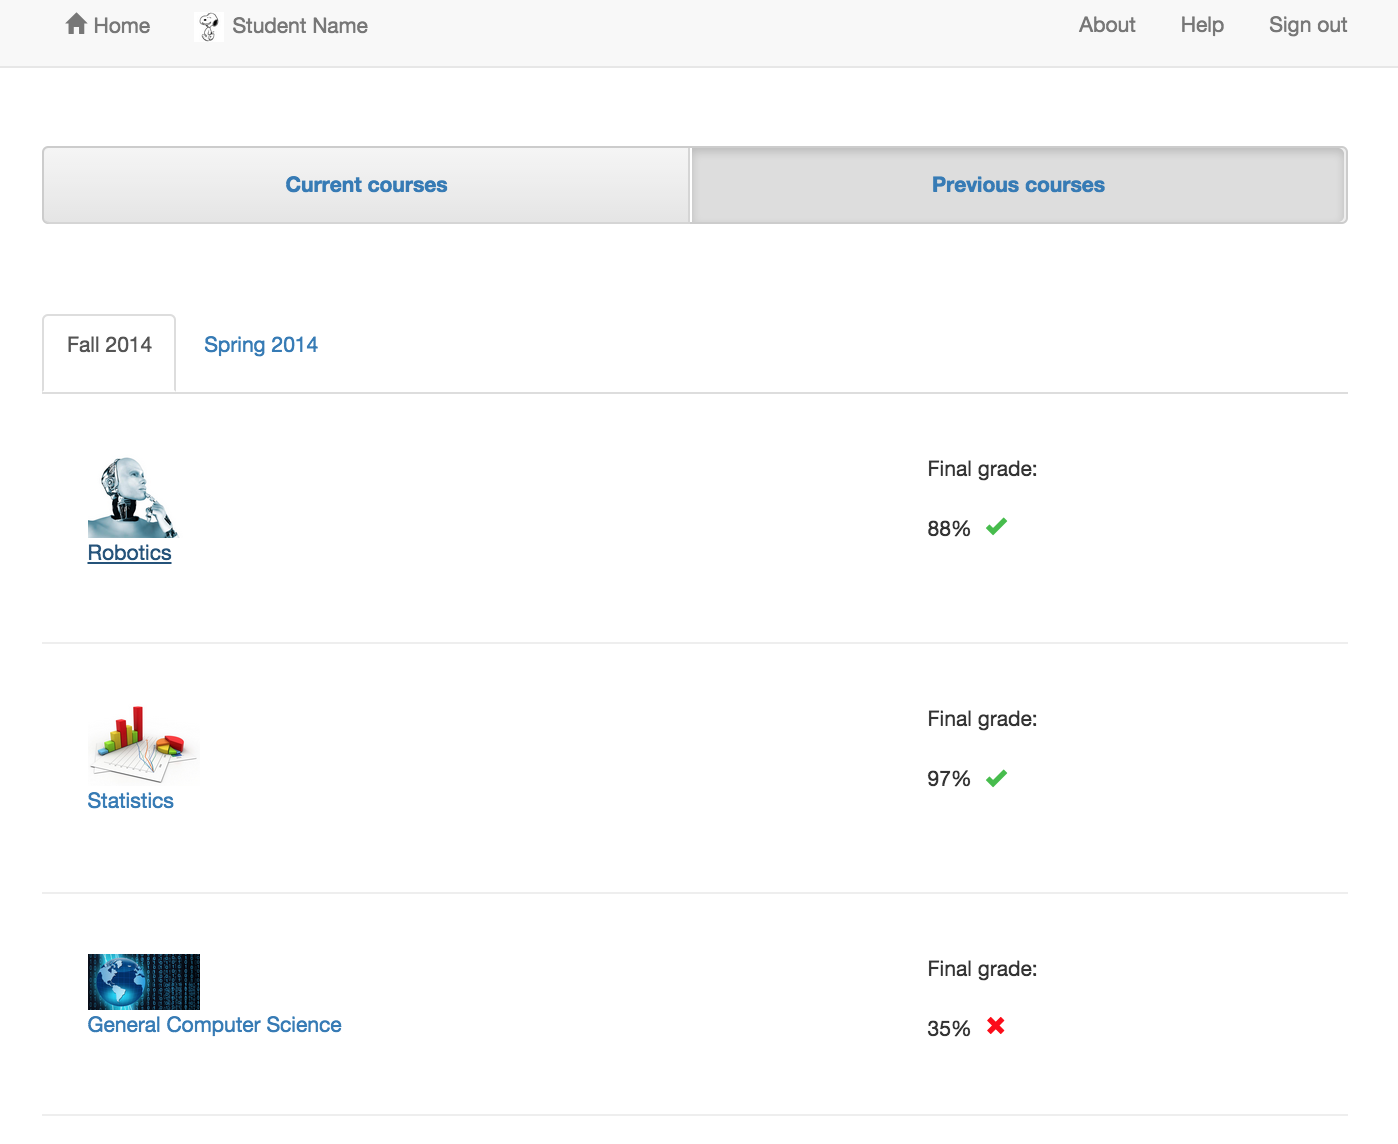
\includegraphics[width=.6\textwidth]{screenshots/PrevoiusCoursesOverview.png}
\newpage
After the student clicks on a course:

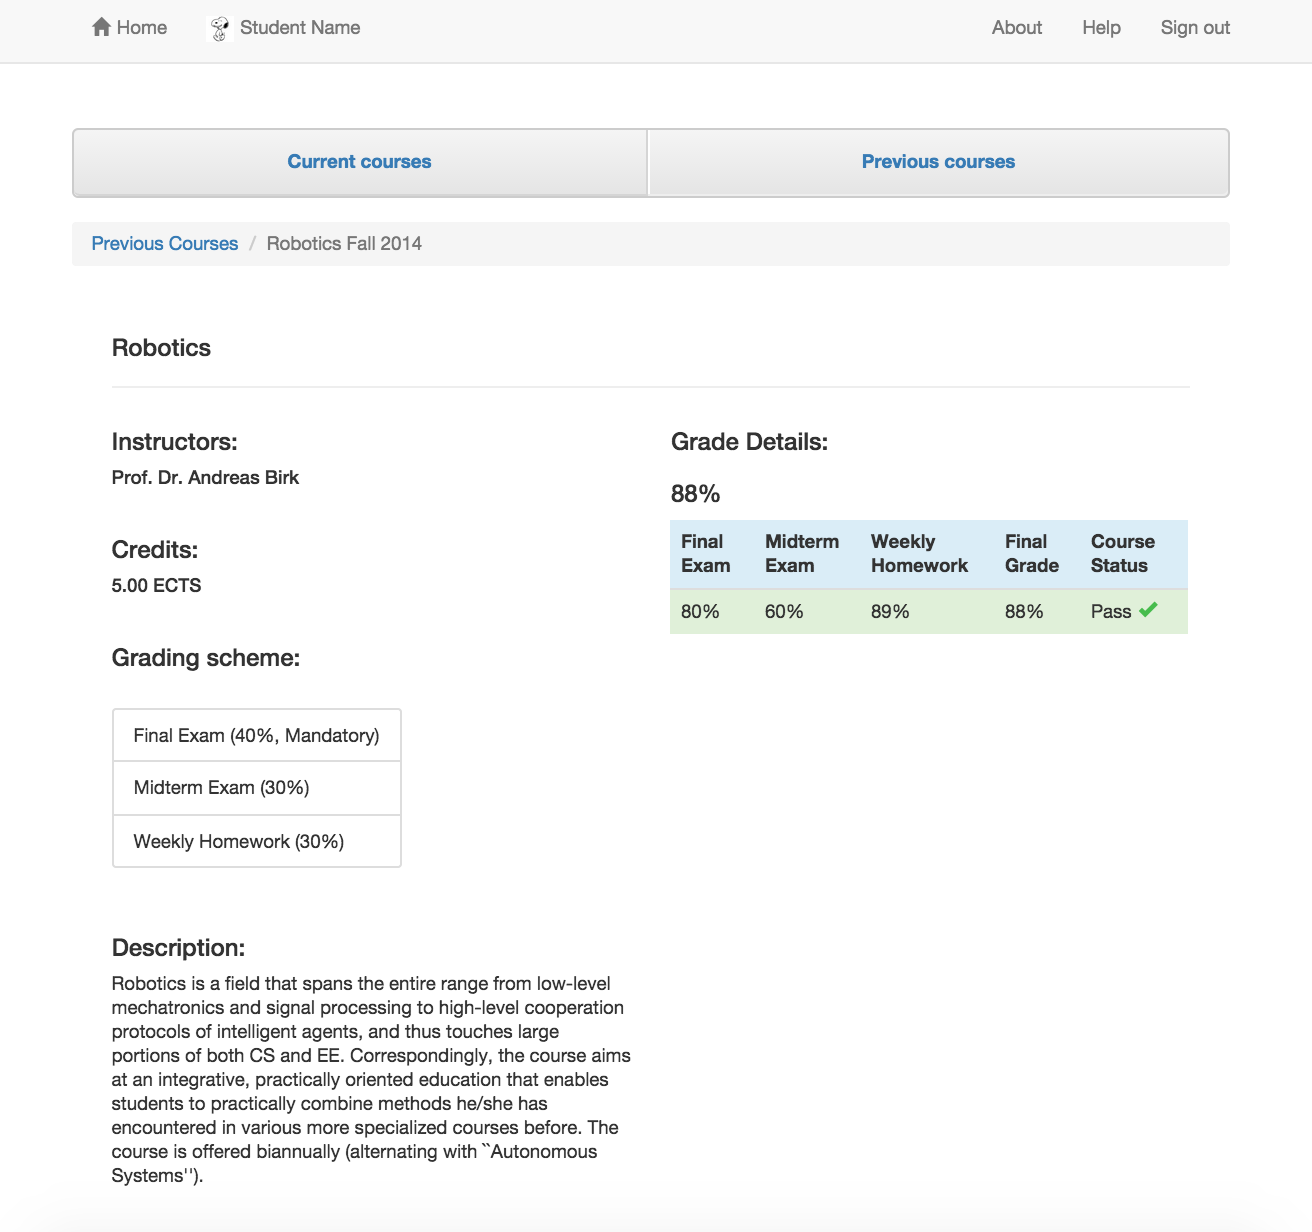
\includegraphics[width=\textwidth]{screenshots/PreviousCourseDetail.png}
\newpage
The student can see the instructor, how may credits he got for the course, grading scheme and the description. We show in a table the grade components and the score he got for each of them. We use green as background for passes course and red for a course which has been failed.

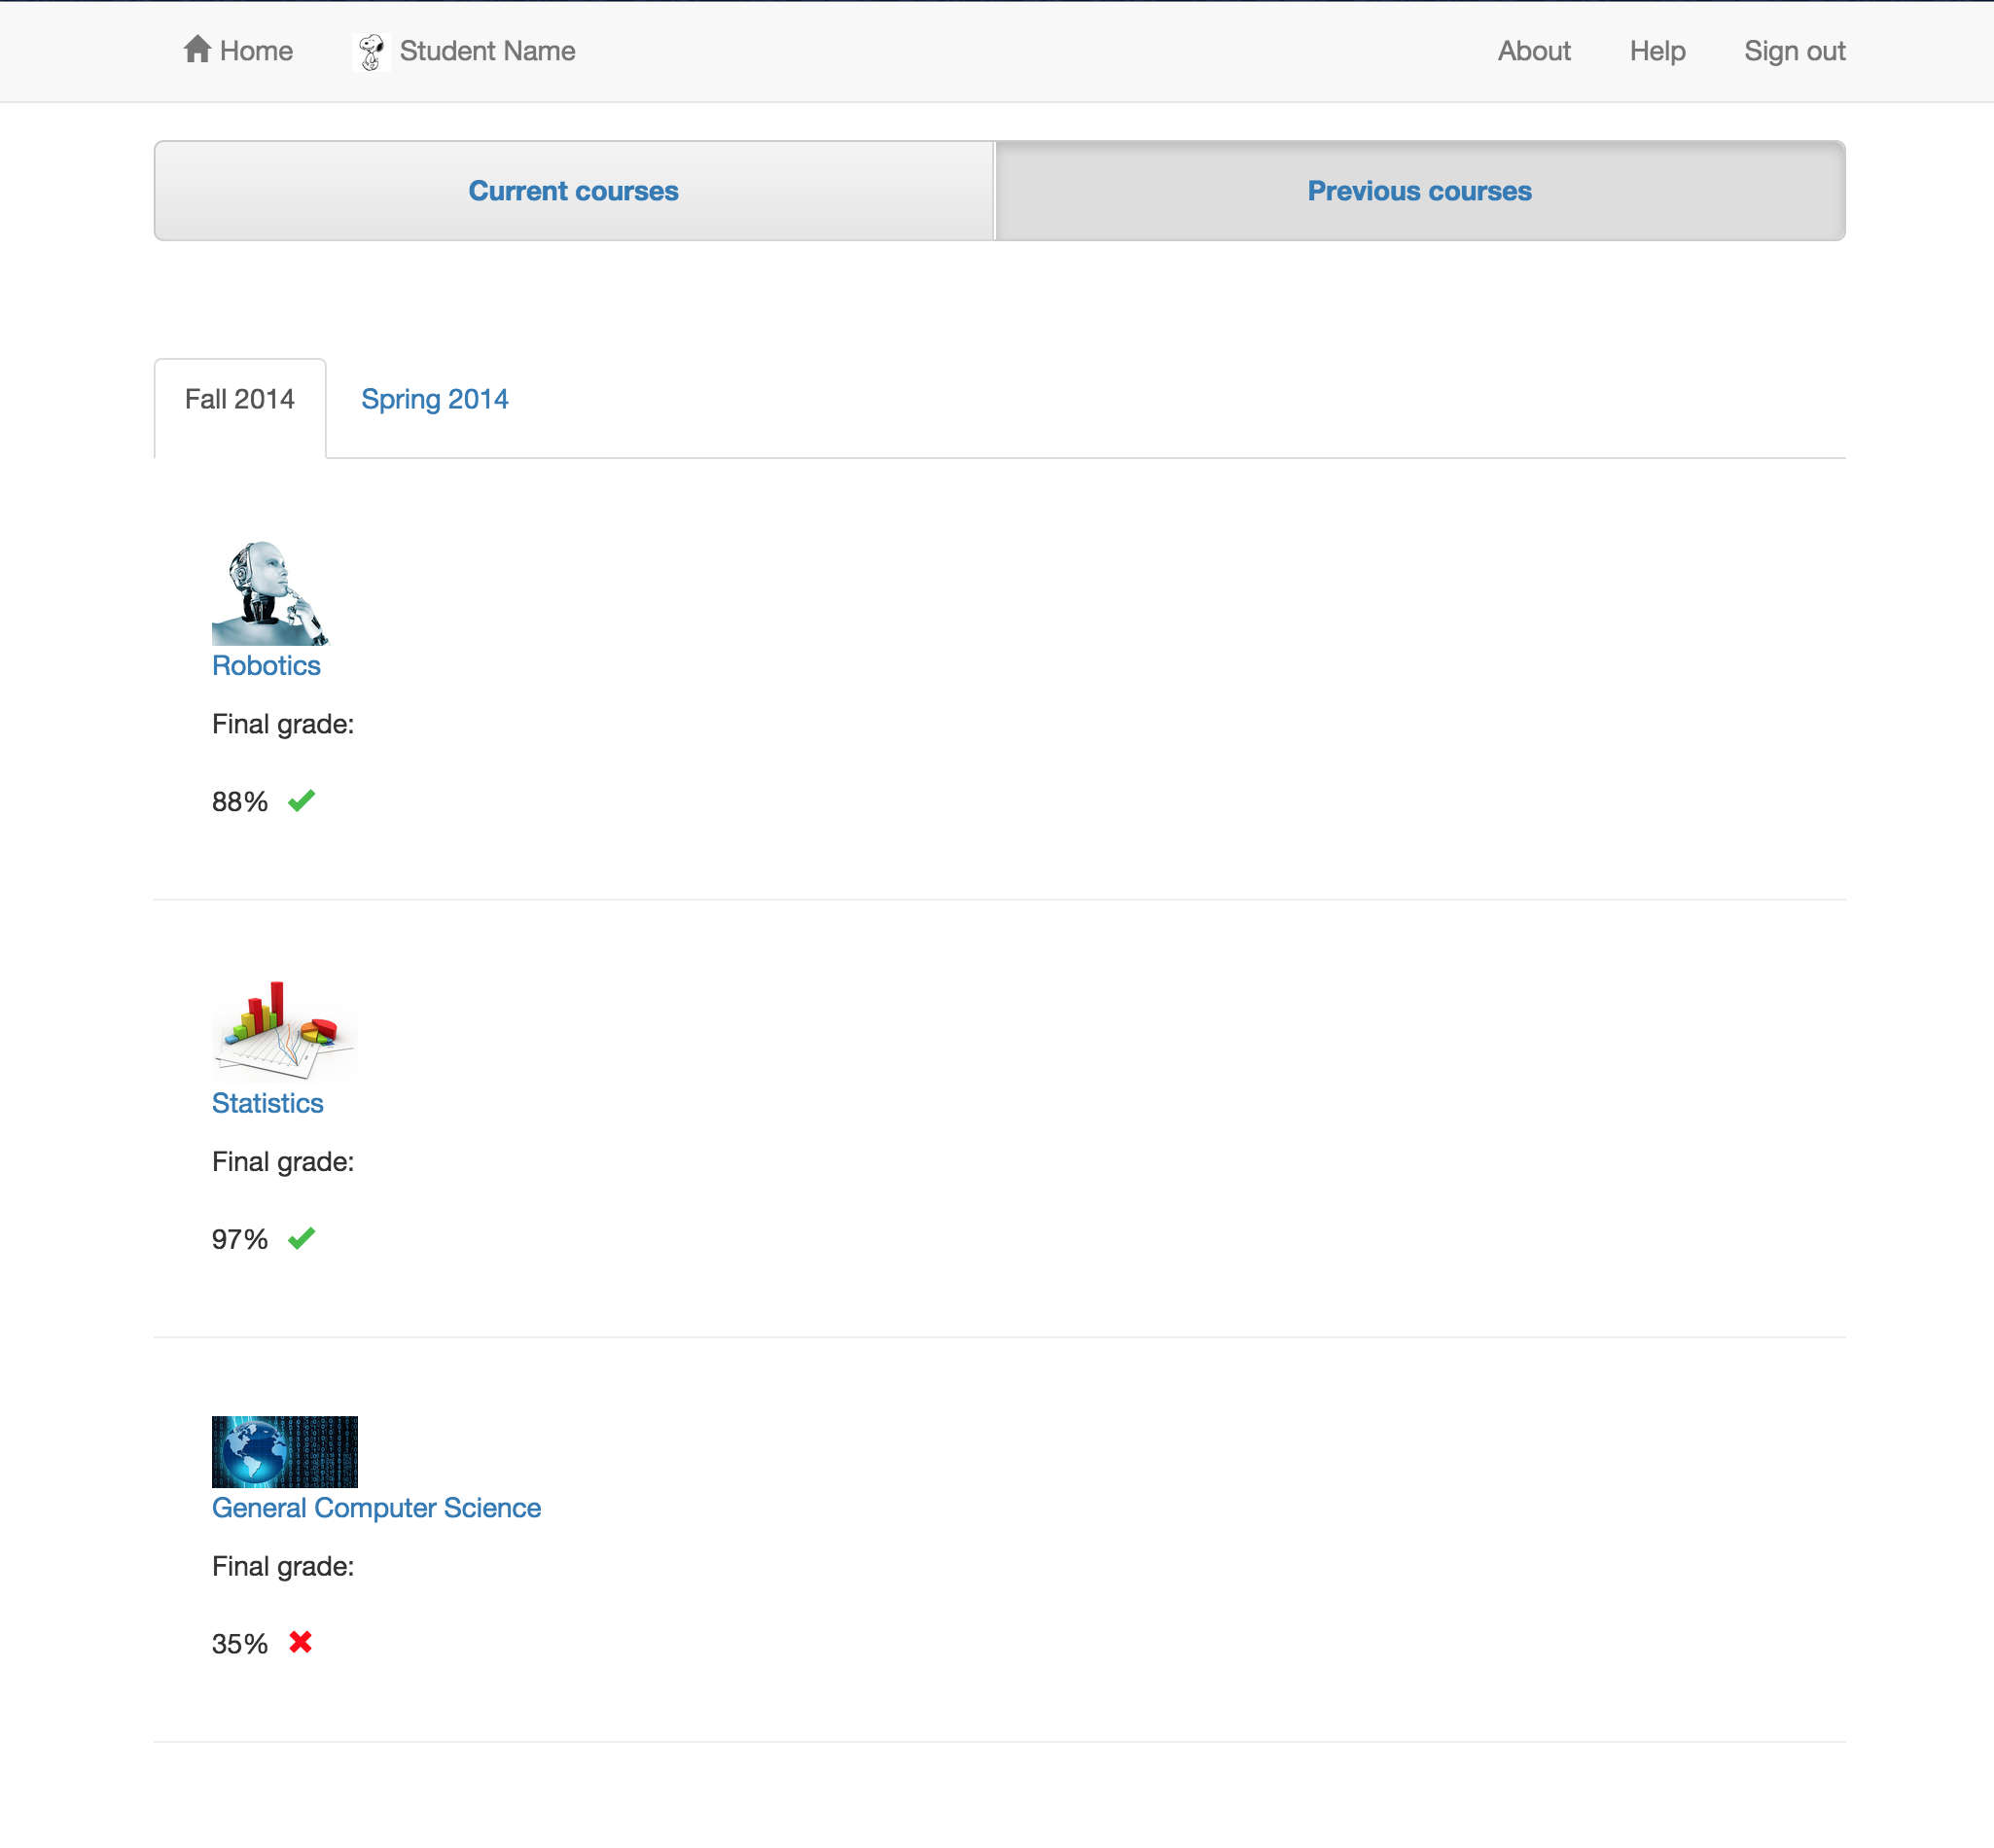
\includegraphics[width=.85\textwidth]{screenshots/PreviousCourses.png}
